\documentclass[conference,a4paper]{IEEEtran}
\IEEEoverridecommandlockouts
%Template version as of 6/27/2024

% --- Packages provided by the IEEE conference template ---
\usepackage{cite}
\usepackage{amsmath,amssymb,amsfonts}
\usepackage{graphicx}
\usepackage{textcomp}
\usepackage{xcolor}

% --- Additional packages required by this paper's content ---
\usepackage{hyperref}
\usepackage{booktabs}
\usepackage{threeparttable}

% Figures live in ../images and ../figures relative to this template directory.
\graphicspath{{../}{../images/}{../figures/}}

\def\BibTeX{{\rm B\kern-.05em{\sc i\kern-.025em b}\kern-.08em
    T\kern-.1667em\lower.7ex\hbox{E}\kern-.125emX}}

\setcounter{secnumdepth}{3}

\begin{document}

\title{Reward Shaping and Terrain-Relative Termination for PPO Humanoid Locomotion Beyond Flat Ground}

\author{\IEEEauthorblockN{Francisco Pinto}
\IEEEauthorblockA{\textit{Faculty of Engineering} \\
\textit{University of Porto (FEUP)}\\
Porto, Portugal \\
up199504009@edu.fe.up.pt}
\and
\IEEEauthorblockN{João Vieira}
\IEEEauthorblockA{\textit{Faculty of Engineering} \\
\textit{University of Porto (FEUP)}\\
Porto, Portugal \\
up202107689@edu.fe.up.pt}
}

\maketitle

\begin{abstract}
Humanoid locomotion is a challenging reinforcement learning problem due to high-dimensional actuation, intermittent contacts, and strong sensitivity to task and environment design. While policy-gradient methods such as Proximal Policy Optimization (PPO) reliably learn flat-ground walking, extending the same recipe to uneven terrain and long-horizon navigation frequently fails in practice, and the causes are often implementation-level rather than algorithmic. We present an empirical case study of two such design choices---reward alignment and episode-termination logic---using the MuJoCo Humanoid across four tasks of increasing difficulty: flat locomotion, stair climbing, waypoint-based circuit navigation, and circuits with stair segments. Task-aligned shaping (height progress and step milestones) yields a stair-climbing policy that reaches the top step in 96\% of evaluation episodes, whereas naive forward-velocity rewards fail on the same terrain. On the combined circuit-with-stairs task, fixed world-frame termination bounds repeatedly prevented learning by terminating healthy agents on elevated terrain; replacing them with a terrain-relative health check enabled 87\% circuit completion. All findings are reported transparently from single-seed final runs with 100-episode evaluations, and the environments, training configurations, and evaluation scripts are publicly released for reproduction.
\end{abstract}

\begin{IEEEkeywords}
Reinforcement Learning, Humanoid Locomotion, MuJoCo, Stair Climbing, Navigation.
\end{IEEEkeywords}

\section{Introduction}

Reinforcement learning (RL) provides a general framework for sequential decision-making in which an agent learns a policy that maximizes cumulative reward through interaction with an environment~\cite{sutton2018reinforcement}. While RL has demonstrated strong performance on simulated continuous-control benchmarks, humanoid locomotion remains particularly challenging due to high-dimensional actuation, intermittent contacts, and sensitivity to environment and task design. Recent humanoid systems, such as Boston Dynamics' Atlas~\cite{bostondynamics2024atlas} and Unitree's H1~\cite{unitree2024h1}, exhibit dynamic locomotion behaviors that are typically supported by extensive simulation training and large-scale computation. Yet even in simulation, policies that perform well on flat terrain frequently fail when extended to uneven terrain or long-horizon navigation, and in our experience this gap is rarely explained by the algorithm alone.

In this work we focus on two implementation-level choices that repeatedly emerged as critical failure points when moving beyond flat locomotion: \emph{reward design} and \emph{termination criteria}. Reward functions that suffice for flat walking often provide weak or misleading learning signals on contact-rich terrain such as stairs. Similarly, termination logic tuned to a fixed ground reference can terminate episodes prematurely when the agent stands on elevated terrain, silently preventing learning.

\begin{figure}[t]
    \centering
    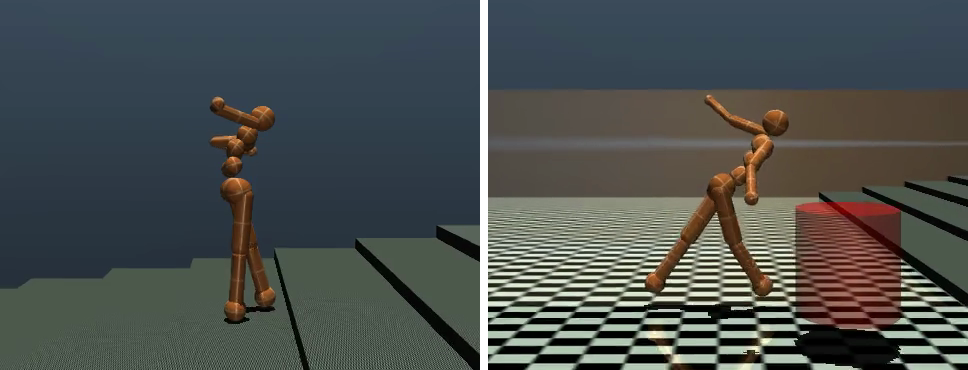
\includegraphics[width=\linewidth]{images/task_environments.png}
    \caption{Trained policies in the two custom environments: stair ascent in \texttt{HumanoidStairsConfigurable-v0} (left) and waypoint navigation toward a marked waypoint with a stair segment ahead in \texttt{HumanoidCircuit-v0} (right).}
    \label{fig:tasks}
\end{figure}

This paper presents an empirical study of these issues using the MuJoCo Humanoid~\cite{todorov2012mujoco,towers2024gymnasium} and PPO~\cite{schulman2017ppo} as implemented in Stable-Baselines3~\cite{raffin2021sb3}. We evaluate a sequence of tasks of increasing complexity: flat locomotion, stair climbing, waypoint-based circuit navigation, and circuits that include stair segments (Fig.~\ref{fig:tasks}). Rather than proposing a new algorithm, our objective is to identify which \emph{implementation-level design decisions} most strongly affect learning stability and task success in this setting. Our contributions are empirical and practitioner-oriented:
\begin{itemize}
    \item Two custom, fully parameterized MuJoCo environments: a configurable stairs environment and a waypoint-based circuit environment with optional stair segments.
    \item A structured comparison of four PPO configurations (S1--S4) that progressively introduce reward shaping, navigation structure, and terrain-aware termination handling.
    \item A transparent evaluation protocol reporting task-completion success rates over 100 episodes per task, alongside an honest account of what our single-seed evidence can and cannot support.
\end{itemize}
For reproducibility, the full implementation---environments, training and evaluation scripts, and the exact per-run configurations---is publicly available at \url{https://github.com/ghostcat-pro/rl-humanoid.git}.

\section{Related Work}
\label{sec:related}

Deep RL has produced locomotion behaviors for simulated humanoids from simple reward signals in rich environments~\cite{heess2017emergence}, and reference-motion methods such as DeepMimic~\cite{peng2018deepmimic} demonstrated that seemingly minor implementation choices---notably \emph{early termination}---can dominate learning outcomes for physics-based characters. Our study extends this line of implementation-focused analysis to terrain-aware termination in torque-controlled humanoid locomotion.

For legged robots, RL controllers trained in simulation have achieved agile and robust locomotion on challenging real terrain, typically using privileged terrain information or teacher--student distillation on quadrupeds~\cite{hwangbo2019agile,lee2020learning,miki2022wild} and massively parallel simulation~\cite{rudin2022minutes,makoviychuk2021isaac}. For bipeds, sim-to-real RL has produced blind stair traversal on Cassie~\cite{siekmann2021stairs}, and causal-transformer policies trained with large-scale RL have controlled a full-scale humanoid outdoors~\cite{radosavovic2024humanoid}. These systems target hardware deployment with substantial engineering pipelines; in contrast, we deliberately isolate two design factors in a controlled, fully observable simulation setting on a standard benchmark humanoid, where their individual effect on learning can be observed directly.

Reward shaping has a long theoretical history~\cite{ng1999shaping}, but task-specific shaping for contact-rich locomotion remains largely empirical; we document which shaping terms were necessary at each task level. Finally, our reporting follows the concerns raised about statistical rigor in deep RL evaluation~\cite{henderson2018matters,agarwal2021precipice}: we state explicitly that final results come from one seed per task and quantify evaluation variability with 100-episode success rates rather than small-sample reward statistics.

\section{Problem Setup}
\label{sec:mdp}

We formalize each task as a Markov Decision Process $(\mathcal{S}, \mathcal{A}, P, r, \gamma)$ with discount $\gamma = 0.99$, solved by a stochastic policy $\pi_\theta(a \mid s)$ trained to maximize the expected discounted return. Transition dynamics $P$ are determined by the MuJoCo physics configuration of each environment (Section~\ref{sec:environments}).

\subsubsection{State Space}
At each control step $t$ the agent receives an observation $o_t$ used as the state. The base observation is \emph{proprioceptive}: joint positions and velocities, torso pose and velocities, and contact forces, following the standard MuJoCo Humanoid convention~\cite{towers2024gymnasium}. The global $(x,y)$ position is excluded in all configurations. Tasks requiring exteroception augment the observation with a local terrain height grid and waypoint-relative navigation features (Section~\ref{sec:obs_design}).

\subsubsection{Action Space}
The action space is continuous, $a_t \in \mathbb{R}^{17}$: torque commands bounded by $[-0.4, 0.4]$ for the 17 actuated hinge joints of the humanoid (3 abdomen, 3 per hip, 1 per knee, 2 per shoulder, 1 per elbow). All environments use a physics timestep of $0.003$\,s with frame skip 5, i.e., a control interval of $dt = 0.015$\,s ($\approx 66.7$\,Hz).

\subsubsection{Episode Termination}
\label{sec:termination}
Episodes end by \emph{truncation} (time limit: 1000 steps for flat locomotion and stairs, 5000 for circuit tasks) or \emph{termination} (health violation). Health is a function of torso height $z_t$: in the baseline, the agent is unhealthy when $z_t$ leaves a fixed world-frame range $[z_{\min}, z_{\max}]$. On elevated terrain this produces false terminations even when the agent is standing upright. Configurations S2 and S4 therefore apply the health range to a \emph{terrain-relative} height
\begin{equation}
\label{eq:terrain_rel_z}
z_{\mathrm{rel},t} = z_t - h(x_t, y_t),
\end{equation}
where $h(x_t, y_t)$ is the terrain height at the agent's planar position. This mechanism is central to our results on combined terrain.

\section{Environments and Tasks}
\label{sec:environments}

We study four tasks of increasing difficulty:
\begin{enumerate}
    \item \textbf{S1, Flat locomotion:} forward walking on flat ground (\texttt{Humanoid-v5}), the standard Gymnasium benchmark, used as a control condition.
    \item \textbf{S2, Stair climbing:} ascend a staircase (\texttt{HumanoidStairsConfigurable-v0}), parameterized by approach distance, number of steps, step height/depth, and top platform. The reported run uses 8 steps of height $0.10$\,m and depth $0.8$\,m; development runs spanned 8--15 steps and heights $0.10$--$0.20$\,m. An episode is successful if the agent reaches the top step.
    \item \textbf{S3, Circuit navigation (flat):} visit a sequence of planar waypoints in order (\texttt{HumanoidCircuit-v0}). The reported course has four waypoints forming a rectangular loop with three turns; success requires reaching all waypoints.
    \item \textbf{S4, Circuit with stairs:} the same environment with a three-waypoint course that includes a five-step stair segment ($0.10$\,m rise) between the first two waypoints.
\end{enumerate}
Side walls constrain circuit courses to a corridor, preventing trivial obstacle bypassing. Beyond flat locomotion, these tasks compound several difficulties: multi-objective coordination (progress, heading, obstacle traversal, energy), sparse milestone rewards atop dense locomotion signals, contact discontinuities at stair edges, and accurate turning---a non-trivial control problem for a torque-driven biped.

All custom environments use MuJoCo's \texttt{RK4} integrator with the \texttt{PGS} solver (50 iterations), terrain friction $(1.0, 0.1, 0.1)$, and \texttt{condim=3} terrain contacts; unspecified options remain at MuJoCo defaults. The exact XML and per-run Hydra configurations are in the repository.

\section{Method}
\label{sec:method}

\subsection{Algorithm}
\label{sec:ppo}

We use PPO~\cite{schulman2017ppo} from Stable-Baselines3~\cite{raffin2021sb3}, an on-policy actor--critic method with the clipped surrogate objective
\begin{equation}
\label{eq:ppo}
L^{\mathrm{CLIP}}(\theta) = \hat{\mathbb{E}}_t \!\left[ \min\!\left( \rho_t(\theta)\,\hat{A}_t,\; \mathrm{clip}\!\left(\rho_t(\theta),\, 1{-}\epsilon,\, 1{+}\epsilon\right)\hat{A}_t \right) \right],
\end{equation}
where $\rho_t(\theta)$ is the importance-sampling ratio and $\hat{A}_t$ the GAE advantage ($\lambda = 0.95$, $\epsilon = 0.2$). Table~\ref{tab:hyperparams} lists the training hyperparameters as actually used in the reported runs.

\begin{table}[t]
\caption{PPO training hyperparameters of the reported runs.}
\label{tab:hyperparams}
\centering
\small
\begin{tabular}{@{}lll@{}}
\toprule
\textbf{Parameter} & \textbf{S1} & \textbf{S2--S4} \\
\midrule
Network (MLP, Tanh) & $256 \times 256$ & $256 \times 256$ \\
Learning rate & $2.5 \times 10^{-4}$ & $3 \times 10^{-4}$ \\
Rollout length & 1{,}024 $\times$ 16 envs & 4{,}096 $\times$ 8 envs \\
Minibatch size & 8{,}192 & 16{,}384 \\
Epochs per update & 10 & 10 \\
Entropy / VF coef. & 0.005 / 0.5 & 0.005 / 0.25 \\
Grad.\ clip / $\gamma$ / GAE $\lambda$ & 0.5 / 0.99 / 0.95 & 0.5 / 0.99 / 0.95 \\
Normalization & \multicolumn{2}{c}{VecNormalize (obs.\ \& rewards)} \\
Training budget & 50M steps & 30M--80M steps \\
\bottomrule
\end{tabular}
\end{table}

\subsection{Observation Design}
\label{sec:obs_design}

All configurations share the proprioceptive base observation. Task-specific augmentations are introduced progressively.

\subsubsection{Terrain Grid (S2--S4)} A local terrain map of 25 samples ($5 \times 5$ offsets) centered on the agent:
\begin{equation}
\label{eq:terrain_grid}
g_t(i,j) = h(x_t + \delta_i,\, y_t + \delta_j) - z_t,
\end{equation}
with fixed world-frame offsets $\delta_i, \delta_j \in \{-0.6, -0.3, 0, 0.3, 0.6\}$\,m; heights are encoded relative to the agent's current $z_t$.

\subsubsection{Waypoint Features (S3, S4)} Navigation state is a 5-dimensional vector
\begin{equation}
\label{eq:waypoint_signal}
w_t = \Big[\,\Delta x_t,\;\Delta y_t,\;\tfrac{n_t}{N_{\mathrm{wp}}},\;\sin(\epsilon_t),\;\cos(\epsilon_t)\,\Big],
\end{equation}
where $(\Delta x_t, \Delta y_t)$ is the displacement to the active waypoint, $n_t/N_{\mathrm{wp}}$ the fraction of completed waypoints, and $\epsilon_t$ the heading error between agent yaw and waypoint direction; $\sin/\cos$ encoding avoids the angle-wrap discontinuity at $\pm\pi$. Table~\ref{tab:obs_dims} summarizes observation dimensionality.

\begin{table}[t]
\caption{Observation space dimensions per configuration.}
\label{tab:obs_dims}
\centering
\small
\begin{tabular}{@{}lcccc@{}}
\toprule
\textbf{Component} & \textbf{S1} & \textbf{S2} & \textbf{S3} & \textbf{S4} \\
\midrule
Proprioceptive core & 348 & 348 & 348 & 348 \\
Additional proprioceptive signals & --- & 28 & 28 & 28 \\
Terrain grid $g_t$ & --- & 25 & 25 & 25 \\
Waypoint features $w_t$ & --- & --- & 5 & 5 \\
\midrule
\textbf{Total} & \textbf{348} & \textbf{401} & \textbf{406} & \textbf{406} \\
\bottomrule
\end{tabular}

\vspace{2pt}
{\raggedright\footnotesize The custom environments expose 28 extra channels (world-body inertia, COM velocity, contact-force, and root actuation signals) beyond the 348-dimensional \texttt{Humanoid-v5} base observation.\par}
\end{table}

\subsection{Reward Design}
\label{sec:reward_design}

The reward optimized by PPO is a task-specific environment reward $r_t^{\mathrm{env}}$ plus a shaping wrapper common to all configurations:
\begin{equation}
\label{eq:total_reward}
r_t^{\mathrm{total}} = r_t^{\mathrm{env}} + \underbrace{w_u \max(0, u_t)}_{\text{upright}} - \underbrace{w_e \|a_t\|_2^2}_{\text{effort}} - \underbrace{w_\ell |y_t|}_{\text{lateral}},
\end{equation}
where $u_t = q_{w}^2 - q_{x}^2 - q_{y}^2 + q_{z}^2$ measures torso uprightness from the (scalar-first) torso quaternion $q$ and $y_t$ is the signed lateral deviation from the corridor centerline. Wrapper weights are $w_u = 0.5$, $w_e = 0.001$, and $w_\ell = 1.0$ ($0.3$ in S2).

\subsubsection{S1: Baseline} The standard \texttt{Humanoid-v5} reward,
\begin{equation}
\label{eq:s1_reward}
r_t^{\mathrm{env}} = \underbrace{w_h \mathbb{1}\!\left[z_{\min} {<} z_t {<} z_{\max}\right]}_{\text{healthy}} + \underbrace{w_f \dot{x}_t}_{\text{forward}} - \underbrace{w_c \lVert a_t \rVert_2^2}_{\text{ctrl}} - c_t^{\mathrm{cf}},
\end{equation}
with $w_h = 5$, $w_f = 1.25$, $w_c = 0.1$, and a contact-force cost $c_t^{\mathrm{cf}} = w_{\mathrm{cf}}\min(\lVert F_{\mathrm{ext}} \rVert_2^2, 10)$, $w_{\mathrm{cf}} = 5 \times 10^{-7}$, capped so rare impact spikes cannot dominate.

\subsubsection{S2: Stairs} Climbing-specific shaping is added:
\begin{equation}
\label{eq:s2_reward}
r_t^{\mathrm{env}} = r_t^{\mathrm{forward}} + r_t^{\mathrm{height}} + r_t^{\mathrm{step}} + r_t^{\mathrm{healthy}} - c_t^{\mathrm{ctrl}} - c_t^{\mathrm{cf}},
\end{equation}
where $r_t^{\mathrm{height}} = w_z \max(0, z_t - z_{t-1})$ rewards upward progress ($w_z = 8$) and $r_t^{\mathrm{step}} = b_s \Delta n_t$ is a milestone bonus for each newly reached stair step ($b_s = 5$). The reported run uses $w_f = 2$, $w_h = 15$, and the terrain-relative health check of Eq.~\eqref{eq:terrain_rel_z} with $z_{\mathrm{rel}} \in [1.0, 2.0]$.

\subsubsection{S3: Waypoint Navigation (Flat)} Forward velocity is replaced by navigation-aligned signals:
\begin{multline}
\label{eq:s3_reward}
r_t^{\mathrm{env}} = r_t^{\mathrm{prog}} + r_t^{\mathrm{dir}} + r_t^{\mathrm{head}} + r_t^{\mathrm{bal}} + r_t^{\mathrm{speed}} \\ + r_t^{\mathrm{bonus}} + r_t^{\mathrm{healthy}} - c_t^{\mathrm{ctrl}} - c_t^{\mathrm{cf}},
\end{multline}
with progress toward the active waypoint $r_t^{\mathrm{prog}} = w_p (d_{t-1} - d_t)$, $w_p = 200$; directional velocity $r_t^{\mathrm{dir}} = w_f \max(0, \dot{\mathbf{x}}^{xy}_t \!\cdot\! \hat{v}_t)$, $w_f = 1$; heading alignment $r_t^{\mathrm{head}} = w_\psi \cos(\epsilon_t) \min(\lVert\dot{\mathbf{x}}^{xy}_t\rVert, 2)$, $w_\psi = 2$ (both active only beyond $0.1$\,m of the waypoint); and sparse bonuses $r_t^{\mathrm{bonus}} = b_{\mathrm{wp}} \mathbb{1}[d_t < \tau] + b_{\mathrm{circ}} \mathbb{1}[\text{all waypoints reached}]$ with $b_{\mathrm{wp}} = 150$, $\tau = 1.5$\,m, $b_{\mathrm{circ}} = 500$. Two regularizers stabilize multi-objective learning:
\begin{equation}
\label{eq:s4_balance_speed}
r_t^{\mathrm{bal}} = w_b \cos\!\Big(\sqrt{\phi_t^2 + \theta_t^2}\Big), \quad
r_t^{\mathrm{speed}} = w_v e^{-\frac{1}{2}\left(\frac{\lVert\dot{\mathbf{x}}_t^{xy}\rVert - v^\star}{\sigma_v}\right)^2},
\end{equation}
rewarding low torso tilt (roll $\phi_t$, pitch $\theta_t$; $w_b = 0.5$) and speeds near a target $v^\star$ ($w_v = 0.2$, $\sigma_v = 0.5$\,m/s; $v^\star = 1.2$\,m/s in S3). S3 runs on flat ground with a world-frame health range.

\subsubsection{S4: Circuit with Stairs} S4 uses the S3 reward with two changes for elevated terrain: the height-progress term from S2 is reintroduced ($w_z = 2$), the speed target is lowered to $v^\star = 1.0$\,m/s, and---critically---termination uses the terrain-relative check of Eq.~\eqref{eq:terrain_rel_z} ($z_{\mathrm{rel}} \in [1.0, 2.0]$, $w_h = 5$). Table~\ref{tab:solutions} summarizes all four configurations.

\begin{table}[t]
\caption{Design choices across configurations S1--S4.}
\label{tab:solutions}
\centering
\small
\begin{tabular}{@{}lcccc@{}}
\toprule
\textbf{Feature} & \textbf{S1} & \textbf{S2} & \textbf{S3} & \textbf{S4} \\
\midrule
Terrain grid observation & --- & \checkmark & \checkmark & \checkmark \\
Height-based climbing term & --- & \checkmark & --- & \checkmark \\
Step milestone bonus & --- & \checkmark & --- & --- \\
Waypoint signals/rewards & --- & --- & \checkmark & \checkmark \\
Balance/speed regularization & --- & --- & \checkmark & \checkmark \\
Terrain-relative termination & --- & \checkmark & --- & \checkmark \\
\bottomrule
\end{tabular}
\end{table}

\section{Results}
\label{sec:results}

\subsection{Protocol}
Development comprised 58 training runs totaling approximately 2.6B environment steps, through which rewards, observations, and termination logic were iterated. The \emph{final} results below come from one training run per task (Table~\ref{tab:final_runs}), each trained independently with seed 42; incremental training across tasks did not reliably preserve previously learned behaviors (Section~\ref{sec:conclusion}). For each task we evaluate the best checkpoint for 100 episodes with a held-out evaluation seed, observation normalization frozen to the training statistics, and rewards reported in raw (unnormalized) units. We report the deterministic policy (mode actions); stochastic-policy results are noted in the text. Success is task-defined: no fall over the full 1000-step horizon (S1), reaching the top step (S2), and reaching all waypoints (S3/S4).

\begin{table}[t]
\centering
\caption{Final training runs (seed 42) and evaluation over 100 episodes per task (deterministic policy, held-out evaluation seed).}
\label{tab:final_runs}
\small
\setlength{\tabcolsep}{4pt}
\begin{threeparttable}
\begin{tabular}{@{}lrrrrr@{}}
\toprule
\textbf{Task} & \textbf{Steps} & \textbf{Ckpt.} & \textbf{Reward} & \textbf{Len.} & \textbf{Success} \\
\midrule
S1: Flat & 50M & 42M & $8{,}429 \pm 2{,}320$ & 912 & 84\% \\
S2: Stairs & 30M & 29M & $15{,}760 \pm 1{,}868$ & 960 & \textbf{96\%} \\
S3: Circuit & 80M & 80M & $6{,}949 \pm 1{,}537$ & 514 & 47\% \\
S4: Circ.+St. & 80M & 64M & $10{,}134 \pm 2{,}421$ & 598 & \textbf{87\%} \\
\bottomrule
\end{tabular}
\begin{tablenotes}[flushleft]
\footnotesize
\item Ckpt.: timestep of the best evaluation checkpoint. Len.: mean episode length (control steps). Success: task-defined completion rate (see text).
\end{tablenotes}
\end{threeparttable}
\end{table}

\begin{figure*}[t]
    \centering
    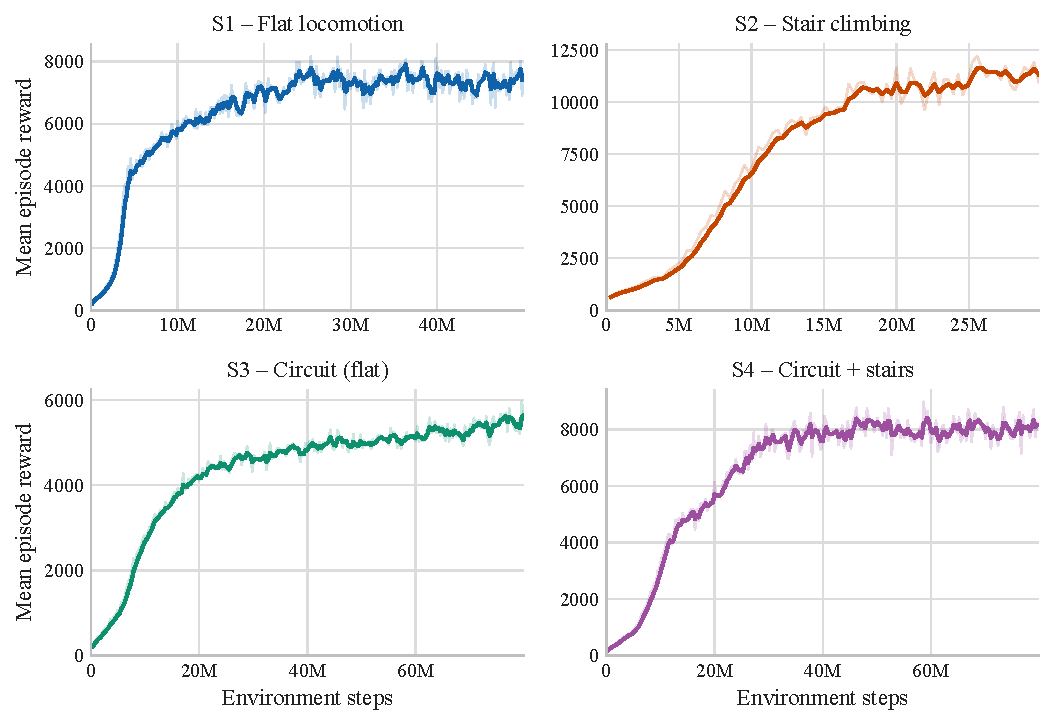
\includegraphics[width=0.92\textwidth]{figures/combined_training_curves.pdf}
    \caption{Training curves for the four final runs: mean episode return per rollout batch in raw reward units (faded: raw; solid: EMA-smoothed). Reward scales are task-specific and not comparable across panels.}
    \label{fig:curves}
\end{figure*}

\subsection{Flat Locomotion (S1)}
The baseline solves flat walking: 84\% of the 100 evaluation episodes complete the full 1000-step horizon without a fall (mean reward $8{,}429 \pm 2{,}320$); the remaining episodes end in late-episode falls. The training curve (Fig.~\ref{fig:curves}, top left) shows rapid initial learning in the first 10M steps and a plateau around $7{,}000$--$7{,}600$ from roughly 25M steps; the best checkpoint was selected at 42M of 50M steps. Under stochastic actions the success rate drops to 29\%, indicating that the learned gait is sensitive to action noise.

\subsection{Stair Climbing (S2)}
With climbing-aligned shaping, the agent reaches the top step in 96\% of episodes (mean reward $15{,}760 \pm 1{,}868$, mean length 960) and then walks stably on the platform. Training (Fig.~\ref{fig:curves}, top right) is the steepest of all configurations: near-asymptotic performance by ${\sim}20$M steps with the best checkpoint at 29M of a 30M budget---the smallest budget among all tasks despite the contact-rich terrain. We attribute this to the dense, well-aligned signal provided by height-progress and step-milestone terms on top of terrain-relative termination.

\subsection{Circuit Navigation, Flat (S3)}
The flat circuit is only partially mastered: the policy reaches on average 3.3 of 4 waypoints, but completes the full course in only 47\% of episodes (mean reward $6{,}949 \pm 1{,}537$; mean length 514 steps). Failures concentrate in the later, sharper turns. Training (Fig.~\ref{fig:curves}, bottom left) rises steadily across the entire 80M-step budget without a clear plateau, and the best checkpoint coincides with the final timestep, suggesting the policy had not converged; the sparse waypoint bonuses provide a weaker signal than the dense forward-velocity and height-progress rewards of S1/S2. Extending training was precluded by the compute budget (Section~\ref{sec:limitations}).

\subsection{Circuit with Stairs (S4)}
The combined task reaches 87\% full-circuit completion---including the stair segment---at a mean reward of $10{,}134 \pm 2{,}421$ and 2.7 of 3 waypoints on average. Training (Fig.~\ref{fig:curves}, bottom right) plateaus near $8{,}000$ from ${\sim}30$M steps with persistent oscillations; the best checkpoint was reached at 64M of 80M steps. We attribute the oscillations to the multi-objective composite reward, in which small degradations of one component (e.g., stair traversal) temporarily depress the total. Note that S4's higher success rate relative to S3 does not imply stairs make navigation easier: the S4 course has three waypoints and one sharp turn versus four waypoints and three turns in S3, so the two success rates are not directly comparable.

Crucially, this configuration \emph{did not learn at all} under fixed world-frame termination: in repeated development runs, otherwise identical setups failed because episodes terminated as soon as the agent stood on elevated terrain, before the stair segment could be mastered. Replacing the world-frame health check with the terrain-relative check of Eq.~\eqref{eq:terrain_rel_z} was the single change that enabled learning. We report this as a consistent qualitative observation rather than a controlled ablation (Section~\ref{sec:limitations}).

\subsection{Convergence and Robustness}
Two cross-task patterns stand out. First, convergence speed tracks reward alignment rather than task simplicity: S2 (stairs) converged fastest despite terrain interaction, while S3 (flat circuit) was slowest, consistent with its sparser milestone signal. Second, training-curve smoothness is a poor predictor of task success: S3 has the smoothest curve but the lowest completion rate (47\%), whereas S4's oscillatory curve yields 87\%. Deterministic-vs-stochastic gaps (84\% vs.\ 29\% on S1; 96\% vs.\ 59\% on S2; 47\% vs.\ 12\% on S3; 87\% vs.\ 41\% on S4) further caution against judging policies by a single evaluation mode.

\section{Conclusions}
\label{sec:conclusion}

We studied how implementation-level design choices govern the transition of PPO-trained humanoid agents from flat locomotion to stair climbing and long-horizon waypoint navigation, and draw three practitioner-oriented findings.

\textbf{Reward design must be task-aligned.} Forward-velocity rewards suffice on flat ground but fail on contact-rich terrain; explicit height-progress and step-milestone terms produced a 96\%-success stair climber with the smallest training budget of all tasks. Conversely, the sparse waypoint bonuses of the circuit task yielded the slowest learning and lowest completion.

\textbf{Termination logic is a first-class design decision.} The clearest failure mode we encountered was not algorithmic: fixed world-frame health bounds repeatedly and silently prevented learning on elevated terrain, while the terrain-relative check of Eq.~\eqref{eq:terrain_rel_z} enabled 87\% completion on the combined task. Termination criteria deserve the same scrutiny as reward terms, echoing early-termination observations in character animation~\cite{peng2018deepmimic}.

\textbf{Naive curriculum transfer is fragile.} Continuing training from a stair-climbing policy into circuit navigation did not preserve earlier skills; without explicit protection, catastrophic forgetting occurred when new objectives were introduced, consistent with known limitations of naive curricula~\cite{bengio2009curriculum}. Final results therefore use independent task-specific runs.

\subsection{Limitations}
\label{sec:limitations}
All final results come from a single seed per task; given known seed sensitivity in deep RL~\cite{henderson2018matters,agarwal2021precipice}, the quantitative values should be read as a documented case study rather than population estimates, and the termination finding as a repeated qualitative observation rather than a controlled, multi-seed ablation. Each run required roughly 3 hours, and iterating rewards and hyperparameters across four tasks consumed the available budget (58 runs, ${\sim}2.6$B steps), precluding per-task sweeps. The policies also rely on privileged terrain height grids, limiting direct sim-to-real transfer, and generalization to unseen stair geometries and external perturbations was not systematically tested. Hyperparameters additionally differ between S1 and S2--S4 (Table~\ref{tab:hyperparams}), a historical artifact of sequential development.

\subsection{Future Work}
Priorities are multi-seed campaigns with a controlled termination ablation, replacing privileged height grids with depth-based perception, domain randomization over terrain geometry, and skill-preservation mechanisms (modular or constrained policies) for multi-task learning. The repository additionally provides functional SAC~\cite{haarnoja2018sac} and TorchRL~\cite{bou2024torchrl} pipelines as starting points.

\bibliographystyle{IEEEtran}
\bibliography{../references}

\end{document}
